\chapter{Introducci\'on}
\label{sec:intro}
%tesis en linguistica http://elies.rediris.es/miscelanea/misce_9/alcina.pdf

%En este cap\'itulo daremos una introducci\'on al problema de la generaci\'on autom\'atica de expresiones referenciales, contaremos las contribuciones de este trabajo y mostraremos como est\'a organizada la tesis.


La {\bf generaci\'on de lenguaje natural (GLN)} es el proceso de construcci\'on de un texto en lenguaje natural de forma autom\'atica (o semi autom\'atica), para la comunicaci\'on con fines espec\'ificos. Este proceso que convierte informaci\'on a texto en lenguaje natural, es \'util para aplicaciones pr\'acticas en las que, por ejemplo, es necesario hacer accesible grandes vol\'umenes de informaci\'on posiblemente t\'ecnica. La GLN se ha usado para generar recomendaciones de restaurantes personalizadas, resumir informaci\'on m\'edica, etc.~\cite{dale2000}. La generaci\'on de lenguaje natural, est\'a dentro de el \'area de procesamiento del lenguaje natural, que es una rama principal de la inteligencia artificial.

La \textbf {generaci\'on de expresiones referenciales (GER)} entre todas las subtareas de GLN, es una de las que ha recibido m\'as atenci\'on. En la pr\'actica, la mayor\'ia de los sistemas GLN, con independencia de su finalidad, contiene un m\'odulo GER de alg\'un tipo~\cite{Mellish2004}. Esto no es sorprendente
en vista del papel central que las expresiones referenciales tienen en la comunicaci\'on. Un sistema que proporciona
consejos sobre los viajes a\'ereos \cite{white2010generating} tiene que hacer referencia a los vuelos --- {\it el
vuelo m\'as barato}, {\it un vuelo directo}---, un sistema de navegaci\'on para autom\'oviles~\cite{Drager:2012:GLN:2380816.2380908}
necesita generar descripciones espaciales ---{\it tomar el puente junto a la iglesia, a la derecha}---,
y un robot que ensambla piezas de juguetes junto con un usuario humano~\cite{foster-etal-ijcai2009} debe hacer referencia a los componentes --- {\it inserte el perno verde hasta el final en el cubo rojo}. Cuando hablamos, nos referimos a cosas (tangibles como un puente, o intangibles como una fecha), es decir generamos expresiones referenciales. Un sistema que genera texto, tambi\'en deber\'a generar expresiones referenciales. La generaci\'on autom\'atica de expresiones referenciales es el tema de esta tesis.

Una {\bf expresi\'on referencial (ER)} es un sintagna nominal que identifica un\'ivocamente a un objeto en un contexto y para un interlocutor particular. Si quisieramos referirnos al objeto se\~nalado por la flecha en la Figura~\ref{GRE3D7-stimulus1}, podr\'iamos hacerlo con alguna de las expresiones referenciales que se muestran en la Figura \ref{er-figura1}.
%\captionsetup{
%  font=footnotesize,
%  justification=raggedright,
%  singlelinecheck=false
%}
\begin{figure}[H]
\begin{subfigure}{.5\textwidth}
  \centering
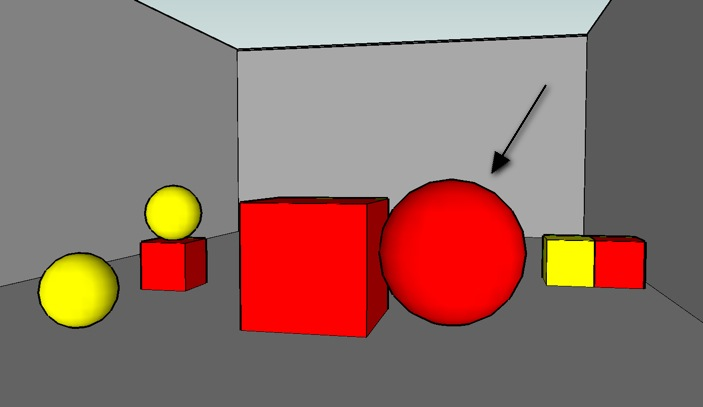
\includegraphics[width=\textwidth]{images/22sinletras.jpg}
  \caption{}\label{GRE3D7-stimulus1}
\end{subfigure}%
\begin{subfigure}{.5\textwidth}
 \centering
%\vspace*{-5cm}
%\begin{table}

\begin{tabular}{l}
 {\it La esfera grande}\\

 {\it La esfera roja que est\'a al lado del cubo rojo} \\

 {\it El objeto que est\'a al lado del cubo grande}\\

 {\it La bola roja}\\

 {\it La pelota a la izquierda del cubo amarillo}\\

 {\it La bola grande}\\

 {\it La esfera que est\'a a la derecha del cubo rojo y a }\\
{\it la izquierda del cubo amarillo}\\

 {\it La cosa que est\'a a la derecha del cubo del medio}\\

  {\it ...}
 \end{tabular}
%\vspace*{-1cm}
\hspace*{-30cm}
\centering\caption{}\label{er-figura1}
\end{subfigure}
\begin{centering}
\caption{Ejemplos de expresiones referenciales que identifican un\'ivocamente al objeto se\~nalado por la flecha en la im\'agen.}
\label{figura-er}
\end{centering}
\end{figure}

Un sistema de GLN incluye 3 etapas, {\bf determinaci\'on de contenido} ---qu\'e decir--- {\bf lexicalizaci\'on} ---con qu\'e palabras--- y {\bf realizaci\'on ling\"{u}\'istica} ---c\'omo decirlo. La selecci\'on de contenido, elije que informaci\'on incluir en la ER. La lexicalizaci\'on elije que lexemas usar para comunicar el contenido determinado por la etapa anterior. Y la realizaci\'on arma la oraci\'on agregando los art\'iculos, preposiciones, y dem\'as lexemas necesarios y orden\'andolos de forma tal que la frase resultante sea gramaticalmente aceptable. 

Un sistema de GER, tiene esas 3 etapas tambi\'en: la determinaci\'on de contenido ---decide qu\'e propiedades o relaciones del objeto se incluir\'an en la expresi\'on referencial---, la lexicalizaci\'on, ---elije las palabras que se van a usar para nombrar las propiedades y relaciones--- y la realizaci\'on ling\"u\'istica, ---se encarga de armar el sintagma nominal para que sea gramaticalmente correcto.

Por ejemplo, la primer ER de la Figura \ref{figura-er} incluye las propiedades {\it tama\~no} y {\it forma} del objeto se\~nalado por la flecha, lexicalizadas como {\it grande} y {\it esfera} respectivamente y realizadas agregando el art\'iculo {\it la} antes de {\it esfera}, e incluyendo el sustantivo {\it esfera} antes que el adjetivo {\it grande}; formando as\'i el sintagma nominal {\it La esfera grande} que es correcto en espa\~nol. Otra lexicalizaci\'on y realizaci\'on de las mismas propiedades ---es decir, de la misma sem\'antica--- podr\'ia ser {\it La bola de gran tama\~no}. A lo largo de esta tesis usaremos el t\'ermino {\bf expresi\'on referencial} para nombrar la salida de cualquiera de las 3 etapas de la GER. Es decir, llamaremos expresi\'on referencial al conjunto de propiedades y relaciones que refieren un\'ivocamente a un objeto aunque no est\'en lexicalizadas o realizadas.

En lo que sigue introduciremos terminolog\'ia b\'asica, relacionada con la GER que nos servir\'a a lo largo de toda la tesis para entendernos.

El {\bf dominio} de una ER define los tipos de entidades que est\'an siendo contemplados. Por ejemplo el dominio de la Figura \ref{figura-er} son las figuras geom\'etricas en 3 dimensiones. En particular, el dominio incluye cubos y esferas de colores rojo y amarillo, algunas grandes y otras peque\~nas, situadas en un entorno con perspectiva.

El {\bf contexto} de una ER contiene un subconjunto de las entidades del dominio. La Figura \ref{figura-er} muestra un contexto con 7 entidades del dominio, 4 rojas y 3 amarillas. Otros ejemplos son los puntos de referencia visibles en un cierto momento en un camino para el que estamos dando direcciones, un subconjunto de las fotograf\'ias utilizadas en una configuraci\'on experimental, o los ingredientes de cocina que ya se han mencionado en una receta. En un dominio visual, el contexto, incluyendo las propiedades de sus objetos y su configuraci\'on espacial, se puede llamar escena. %El contexto de la Figura \ref{GRE3D7-stimulus1} son los todos los objetos visibles con sus propiedades.

Cada {\bf entidad} del contexto (tambi\'en conocido como objeto o elemento) tiene un tipo ---\emph{esfera}--- ciertas propiedades o caracter\'isticas ---\emph{color}---, valores de esas propiedades ---\emph{rojo}---, y puede tener relaciones con otros objetos ---\emph{a la derecha de}. Una {\bf propiedad} (unaria) es una caracter\'istica de una entidad particular. Por ejemplo, la raza de un perro, el tener o no tener bigotes para un hombre, o el color para un objeto. Cada entidad puede tener muchas propiedades, y puede tener relaciones (tambi\'en llamadas: propiedades binarias), por ejemplo con respecto a la posici\'on f\'isica, como estar situado al lado de otro objeto. 

El {\bf target} (u objetivo), es el subconjunto de objetos de un contexto a los cuales queremos referirnos. En la escena del ejemplo de la Figura \ref{figura-er}, el target es el objeto se\~nalado por la flecha. En este caso, el target es un conjunto singleton, es decir tiene un s\'olo elemento. Si el target tiene m\'as de un elemento, las ER que lo identifican ser\'an plurales.

Dado un contexto, un target y una descripci\'on (parcial) del target, los {\bf distractores} son otros elementos que se encuentran en el contexto, y que tambi\'en cumplen con la descripci\'on parcial. Si la descripci\'on parcial es {\it esfera} las esferas que no son el target de la Figura \ref{GRE3D7-stimulus1} son  distractores, y por ello es necesario seguir agregando propiedades o relaciones para identificar un\'ivocamente al target.

Un {\bf algoritmo} para GER, es un procedimiento autom\'atico que toma, al menos, alg\'un tipo de representaci\'on de un contexto y un target, y d\'a como resultado una (o m\'as) expresi\'on(es) referencial(es) para el target considerado, si puede identificarlo un\'ivocamente en el contexto.
\vspace*{-1.5cm}
\begin{figure}[H]
\begin{subfigure}{.4\textwidth}
  \centering
	\vspace*{-.2cm}
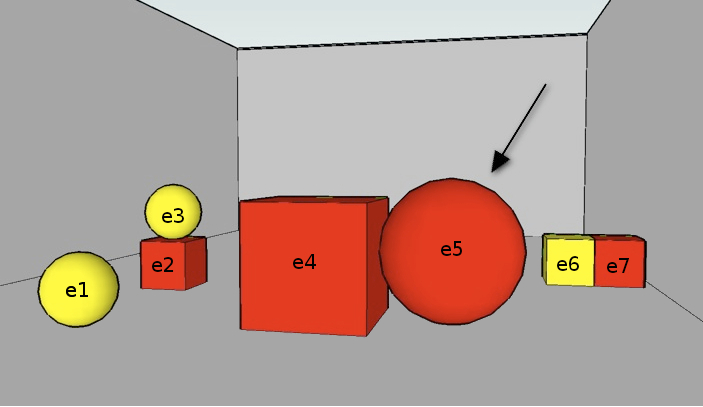
\includegraphics[width=\textwidth]{images/22.jpg}
  \caption{}\label{GRE3D7-stimulus1-ids}
\end{subfigure}
\begin{subfigure}{1\textwidth}
 \centering
\begin{centering}
\hspace*{-6cm}
\begin{scriptsize}
\begin{tabular}{|l|c|c|c|c|c|c|c|}
\hline
\textbf {id}& 	\textbf {type}		&	\textbf {color}	&	\textbf {size}& \textbf {rigth} & \textbf {left} & \textbf {ontop}	& \textbf {below}	\\
   	   &  	    			&	    		&	     		&  \textbf {of}   		 &  \textbf {of}	    &  \textbf {of}	&  \textbf {of}\\
\hline \hline
$e_1$ & ball & yellow & small & - & - & - & - \\
$e_2$ & cube & red & small & - & - &- & $e_3$ \\
$e_3$ & ball & yellow & small & - & - & $e_2$ & -\\
$e_4$ & cube & red & large & - & $e_5$ & - & -\\
$e_5$ & ball & red & large & $e_4$ & - & - & -\\
$e_6$ & cube & yellow & small & - & $e_7$ & - & -\\
$e_7$ & cube & red & small & $e_6$ & - & - & -\\
\hline
\end{tabular}
\end{scriptsize}
\caption{}\label{tabla-propiedades}
\end{centering}
\end{subfigure}
\caption{Posible formalizaci\'on de las propiedades de la Figura \ref{figura-er} en una tabla de doble entrada.}\label{contexto-tabla-propiedades}
\end{figure}

\vspace*{-2cm}Una computadora que se enfrenta a la tarea de generar autom\'aticamente expresiones referenciales en un contexto determinado, necesitar\'a una representaci\'on de todos los objetos y las propiedades de cada uno de ellos. En la Figura~\ref{contexto-tabla-propiedades} se muestra una posible forma de representar los objetos, sus propiedades y relaciones: una base de datos que contiene todas las propiedades relevantes de los objetos de la escena. Entonces, la tarea de GER para el objeto $e_5$ incluye encontrar alguna combinaci\'on de valores de propiedades y relaciones con otros objetos, que aplique \'unicamente a $e_5$, y no a los otros objetos. Esta tarea de encontrar las propiedades y relaciones que aplican a un target y no a los distractores, se llama {\emph selecci\'on de contenido para la generaci\'on de una expresi\'on referencial}.
Como una primera intuici\'on podemos ver que la Figura \ref{formula-subgrafo} es un subrafo de la Figura \ref{representacion-modelo} que identifica un\'ivocamente al target, representa la cuarta ER mostrada en la Figura \ref{er-figura1}. Y la Figura \ref{formula-subgrafo2} tambi\'en identifica al target un\'ivocamente y representa la segunda ER mostrada en \ref{er-figura1}.
%que est\'an dadas en la Figura \ref{er-figura1} son muchas m\'as de las que mostramos en las f\'ormulas de la Figura \ref{er-figura1-b}, esto nos lleva a pensar que un algoritmo puede que no consiga la variedad que las personas dan. La representaci\'on ilustrada en la Figura~\ref{representacion-modelo} es equivalente a la mostrada en la Tabla \ref{tabla-propiedades}.

\begin{figure}[H]
\begin{subfigure}{.5\textwidth}
  \centering
%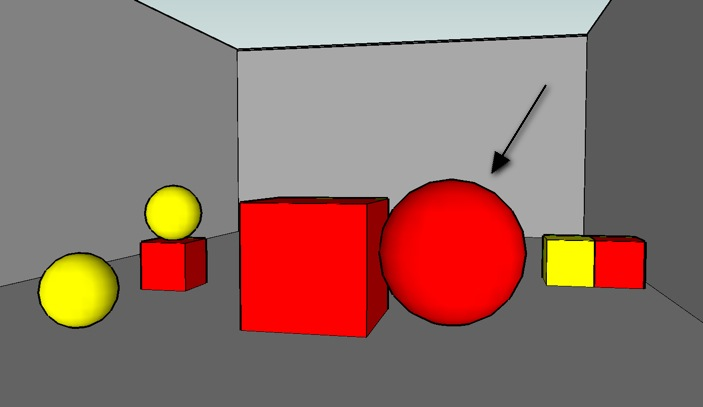
\includegraphics[width=\textwidth]{images/22sinletras.jpg}
%%\caption{Ejemplo de contexto}
%\label{GRE3D7-stimulus1-b}
\vspace*{1cm}
\begin{picture}(250,50)
\put(0,-50){\begin{tikzpicture}
  [
    n/.style={circle,draw,inner sep=1.5pt,node distance=1.5cm},
		 aArrow/.style={->, >=stealth, semithick, shorten <= 1pt, shorten >= 1pt},
  ]
 \node[n,label=below:{
    \relsize{-2}$\begin{array}{c}
      \nSmall\\[-3pt] 
      \nYellow \\[-3pt] 
      \nBall\end{array}$}] (a) {$e_1$};
 \node[n,label=below:{
    \relsize{-2}$\begin{array}{c}     
      \nSmall\\[-3pt] 
      \nRed\\[-3pt] 
      \nCube\end{array}$}, right of=a] (b) {$e_2$};
 \node[n,label=above:{
    \relsize{-2}$\begin{array}{c}     
      \nSmall\\[-3pt] 
      \nYellow\\[-3pt] 
      \nBall\end{array}$}, above of=b] (c) {$e_3$};
 \node[n,label=below:{
    \relsize{-2}$\begin{array}{c}
      \nLarge\\[-3pt] 
      \nRed\\[-3pt] 
      \nCube\end{array}$}, right of=b] (d) {$e_4$};
 \node[n,label=below:{
    \relsize{-2}$\begin{array}{c}
      \nLarge\\[-3pt] 
      \nRed\\[-3pt] 
      \nBall\end{array}$}, right of=d] (e) {$e_5$};
 \node[n,label=below:{
    \relsize{-2}$\begin{array}{c}
      \nSmall\\[-3pt] 
      \nYellow\\[-3pt] 
      \nCube\end{array}$}, right of=e] (f) {$e_6$};
 \node[n,label=below:{
    \relsize{-2}$\begin{array}{c}
      \nSmall\\[-3pt]
      \nRed\\[-3pt] 
      \nCube\end{array}$},  right of=f] (g) {$e_7$};
 \draw [aArrow,bend right=40] (b) to node[auto,swap]{\relsize{-3}$\nBelow$} (c);
 \draw [aArrow,bend right=40] (c) to node[auto,swap]{\relsize{-3}$\nOntop$} (b);
 \draw [aArrow,bend right=40] (d) to node[auto,swap]{\relsize{-3}$\nLeftof$} (e);
 \draw [aArrow,bend right=40] (e) to node[auto,swap]{\relsize{-3}$\nRightof$} (d);
 \draw [aArrow,bend right=40] (f) to node[auto,swap]{\relsize{-3}$\nLeftof$} (g);
 \draw [aArrow,bend right=40] (g) to node[auto,swap]{\relsize{-3}$\nRightof$} (f);
 %\draw[dotted] (-0.5,-1.3) rectangle (8,3.1);
 \draw[dotted] (-0.5,-1.5) rectangle (8,3);
 \end{tikzpicture}}
 \end{picture}
 %\end{flushleft}

\vspace*{2cm} 
 \caption{}\label{representacion-modelo}

\end{subfigure}%
\begin{subfigure}{.6\textwidth}
 \centering
%\hspace*{0cm}
%\vspace*{-5cm}
%\begin{minipage}[t]{0.5\linewidth}
%\centering
%\vspace*{-5cm}
%\begin{table}





%\begin{subfigure}{.5\textwidth}
%  \centering
%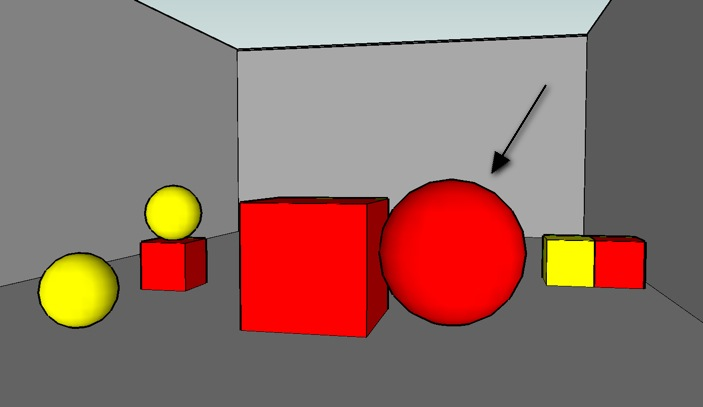
\includegraphics[width=\textwidth]{images/22sinletras.jpg}
%%\caption{Ejemplo de contexto}
%\label{GRE3D7-stimulus1-b}
\centering
%\vspace*{-2cm}
\begin{picture}(190,50)
\put(40,-50){\begin{tikzpicture}
  [
    n/.style={circle,draw,inner sep=1.5pt,node distance=1.5cm},
		 aArrow/.style={->, >=stealth, semithick, shorten <= 1pt, shorten >= 1pt},
  ]
 %\node[n,label=below:{
    %\relsize{-2}$\begin{array}{c}
      %\nRed\\[-3pt] 
      %\nCube\end{array}$}, right of=b] (d) {$e_4$};
 \node[n,label=below:{
    \relsize{-2}$\begin{array}{c}
      \nRed\\[-3pt] 
      \nBall\end{array}$}, right of=d] (e) {$e_5$};

% \draw [aArrow,bend right=40] (d) to node[auto,swap]{\relsize{-3}$\nLeftof$} (e);
 %\draw [aArrow,bend right=40] (e) to node[auto,swap]{\relsize{-3}$\nRightof$} (d);

 %\draw[dotted] (-0.5,-1.3) rectangle (8,3.1);
 %\draw[dotted] (-0.5,1) rectangle (8,3);
 \end{tikzpicture}}
 \end{picture}
 %\end{flushleft}

\vspace*{1.5cm} 
 \caption{Subgrafo $\nBall \land \nRed$} \label{formula-subgrafo}

\vspace*{-1cm}
\begin{picture}(150,50)
\put(10,-50){\begin{tikzpicture}
  [
    n/.style={circle,draw,inner sep=1.5pt,node distance=1.5cm},
		 aArrow/.style={->, >=stealth, semithick, shorten <= 1pt, shorten >= 1pt},
  ]
 \node[n,label=below:{
    \relsize{-2}$\begin{array}{c}
      \nRed\\[-3pt] 
      \nCube\end{array}$}, right of=b] (d) {$e_4$};
 \node[n,label=below:{
    \relsize{-2}$\begin{array}{c}
      \nRed\\[-3pt] 
      \nBall\end{array}$}, right of=d] (e) {$e_5$};

% \draw [aArrow,bend right=40] (d) to node[auto,swap]{\relsize{-3}$\nLeftof$} (e);
 \draw [aArrow,bend right=40] (e) to node[auto,swap]{\relsize{-3}$\nRightof$} (d);

 %\draw[dotted] (-0.5,-1.3) rectangle (8,3.1);
 %\draw[dotted] (-0.5,2) rectangle (8,5);
 \end{tikzpicture}}
 \end{picture}
 %\end{flushleft}

\vspace*{2cm} 
 \caption{Subgrafo $\nBall \land \nRed \land \exists \nRightof . (\nCube  \land \nRed)$} \label{formula-subgrafo2}



\vspace*{0.5cm}
%\begin{tabular}{l}
 %{\it ball and large}\\
%
 %{\it ball and red and Ex.right-of (cube and red)} \\
%
 %{\it Ex.(T) and Ex.right-of (large and cube)}\\
%
 %{\it red and ball}\\
%
%% {\it ball and Ex.left-of (yellow and cube)}\\
%
 %{\it large and ball}\\
%
 %%{\it ball and Ex.right-of (red and cube and}\\
 %%{\it Ex.left-of (yellow cube)}\\
 %%{\it Ex.(T) and Ex.right-of o}\\
%
 %{\it ...}
 %
%
 %\end{tabular}



\vspace*{1cm}

 %\caption{ER como f\'ormulas l\'ogicas para el objeto $e_5$.}\label{er-figura1-b}
%\end{table}
%\end{minipage}
\end{subfigure}%
\caption{Ejemplos de ER en f\'ormulas l\'ogicas para la Figura \ref{GRE3D7-stimulus1-ids}.}
\label{formulas-stimulus1}
\end{figure}






 En la pr\'oxima secci\'on veremos porqu\'e la tarea GER es m\'as compleja de lo que parece a primera vista y en la siguiente introduciremos c\'omo herramientas de teor\'ia de modelos nos pueden ayudar.

\section{Expresiones referenciales bajo incertidumbre}
\label{sec:gre-incertidumbre}


%Los conjuntos son dif\'icil para referirse a, por ejemplo, y algoritmos
%diseñado para tratar con ellos lograr una menor semejanza humana cuando se refiere a los conjuntos de
%a los objetos individuales (van Deemter et al., en prensa). Los recientes esfuerzos para dejar que los algoritmos REG
%referirse a las regiones espaciales sugieren que en dominios grandes, realista, identificación precisa de
%un objetivo es un objetivo que se puede aproximar, pero rara vez alcanzado (Turner et al., 2008;
%Turner, Sripada, y Reiter 2009) .Es en tales dominios que prominencia (especialmente en el
%sentido no lingüístico) se convierte en un problema crítico. 
Cuando la generaci\'on de expresiones referenciales ocurre en la vida real
en lugar de ocurrir en un experimento controlado las fuentes de \textbf{incertidumbre} que afectan al proceso se multiplican. En trabajo 
reciente en el \'area de GER \cite{turner2008}, \cite{turner2009} se discute que, al intentar usar algoritmos de GER en dominios grandes 
y realistas -(como por ejemplo, la descripci\'on de regiones en mapas), la identificaci\'on precisa del target es una tarea que puede ser 
aproximada pero raramente lograda. Los autores argumentan que esto se debe, en parte, a que las representaciones geogr\'aficas 
son necesariamente \textbf{incompletas}. Esta falta de informaci\'on introduce incertidumbre ---por ejemplo ?`es realmente el \'unico restaurant 
de esa calle o es el \'unico que aparece en el mapa?.
Cuando la informaci\'on del contexto proviene de datos de sensores, las entradas del algoritmo de GER son inevitablemente ruidosas. Es decir, 
contienen informaci\'on no s\'olo incompleta sino tambi\'en posiblemente {\bf incorrecta}. Incluso en contextos tan simples como el de la 
Figura \ref{figura-er} hay incertidumbre. ?`Estamos seguros que la Figura \ref{representacion-modelo} representa toda la informaci\'on del 
contexto?. Algunos podemos opinar que s\'i, otros que no. En efecto, la persona que gener\'o la ER {\emph la pelota a la izquierda del cubo 
amarillo} opina que no: la relaci\'on \emph{a la izquierda de} entre el target y el cubo amarillo no est\'a representada en el grafo. Un 
algoritmo de GER con este grafo como input no puede generar esta expresi\'on referencial. El grafo puede completarse para que sea posible
generar la expresi\'on referencial. El grafo resultante se ilustra en la Figura \ref{representacion-modelo-completo}. Sin embargo, este grafo tampoco es completo, 
de hecho, la ER {\emph la cosa que est\'a a la derecha del cubo del medio} no se podr\'ia generar con este grafo. La informaci\'on no s\'olo 
impide la generaci\'on de ER v\'alidas, sino que tambi\'en permite la generaci\'on de ER claramente incorrectas como \emph{la esfera roja 
que no tiene nada a la derecha}.

\begin{figure}[H]
%\begin{subfigure}{.5\textwidth}
\centering
%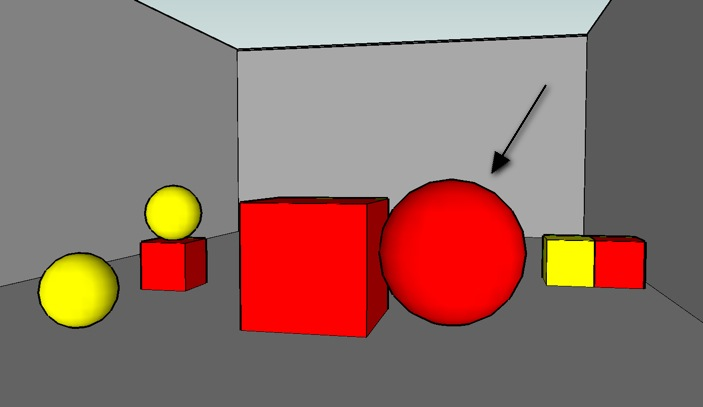
\includegraphics[width=\textwidth]{images/22sinletras.jpg}
%%\caption{Ejemplo de contexto}
%\label{GRE3D7-stimulus1-b}
\vspace*{1cm}
\begin{picture}(250,50)
\put(0,-50){\begin{tikzpicture}
  [
    n/.style={circle,draw,inner sep=1.5pt,node distance=1.5cm},
		 aArrow/.style={->, >=stealth, semithick, shorten <= 1pt, shorten >= 1pt},
  ]
 \node[n,label=below:{
    \relsize{-2}$\begin{array}{c}
      \nSmall\\[-3pt] 
      \nYellow \\[-3pt] 
      \nBall\end{array}$}] (a) {$e_1$};
 \node[n,label=below:{
    \relsize{-2}$\begin{array}{c}     
      \nSmall\\[-3pt] 
      \nRed\\[-3pt] 
      \nCube\end{array}$}, right of=a] (b) {$e_2$};
 \node[n,label=above:{
    \relsize{-2}$\begin{array}{c}     
      \nSmall\\[-3pt] 
      \nYellow\\[-3pt] 
      \nBall\end{array}$}, above of=b] (c) {$e_3$};
 \node[n,label=below:{
    \relsize{-2}$\begin{array}{c}
      \nLarge\\[-3pt] 
      \nRed\\[-3pt] 
      \nCube\end{array}$}, right of=b] (d) {$e_4$};
 \node[n,label=below:{
    \relsize{-2}$\begin{array}{c}
      \nLarge\\[-3pt] 
      \nRed\\[-3pt] 
      \nBall\end{array}$}, right of=d] (e) {$e_5$};
 \node[n,label=below:{
    \relsize{-2}$\begin{array}{c}
      \nSmall\\[-3pt] 
      \nYellow\\[-3pt] 
      \nCube\end{array}$}, right of=e] (f) {$e_6$};
 \node[n,label=below:{
    \relsize{-2}$\begin{array}{c}
      \nSmall\\[-3pt]
      \nRed\\[-3pt] 
      \nCube\end{array}$},  right of=f] (g) {$e_7$};
 \draw [aArrow,bend right=40] (b) to node[auto,swap]{\relsize{-3}$\nBelow$} (c);
 \draw [aArrow,bend right=40] (c) to node[auto,swap]{\relsize{-3}$\nOntop$} (b);
 \draw [aArrow,bend right=40] (d) to node[auto,swap]{\relsize{-3}$\nLeftof$} (e);
 \draw [aArrow,bend right=40] (e) to node[auto,swap]{\relsize{-3}$\nRightof$} (d);
 \draw [aArrow,bend right=40] (f) to node[auto,swap]{\relsize{-3}$\nLeftof$} (g);
 \draw [aArrow,bend right=40] (g) to node[auto,swap]{\relsize{-3}$\nRightof$} (f);
 
 \draw [aArrow,bend right=40] (a) to node[auto,swap]{} (b);
 \draw [aArrow,bend right=40] (b) to node[auto,swap]{} (a);

 \draw [aArrow,bend right=40] (b) to node[auto,swap]{} (d);
 \draw [aArrow,bend right=40] (d) to node[auto,swap]{} (b);

\draw [aArrow,bend right=40] (e) to node[auto,swap]{} (f);
 \draw [aArrow,bend right=40] (f) to node[auto,swap]{} (e);
 %\draw[dotted] (-0.5,-1.3) rectangle (8,3.1);
 \draw[dotted] (-0.5,-1.5) rectangle (8,3);
 \end{tikzpicture}}
 \end{picture}
 %\end{flushleft}

\vspace*{2cm} 
 \caption{Representaci\'on de contexto m\'as completo.}\label{representacion-modelo-completo}
\end{figure}


Aunque no hablemos ni de incompletitud ni de incorrectitud tambi\'en hay incertidumbre en \textbf{cu\'al} de todas las posibles ERs un sistema de GER debe 
elegir. Por ejemplo seguramente hay personas que preferir\'an ERs que usen la palabra {\emph esfera}, antes que {\emph bola}. Y seguramente 
no falte quien diga que {\emph la} mejor expresi\'on referencial ni si quiera aparece en la Figura \ref{figura-er}. Sin embargo, seguramente 
habr\'a una tendencia como se muestra en estudios previos \cite{viet:gene11}. Nadie preferir\'a una ER que use 21 propiedades y 6 relaciones 
para describir al target de la Figura \ref{figura-er}.

El largo de una ER afecta su calidad. Se podr\'{i}a pensar, por ejemplo, que las referencias son \'optimas cuando son {\textbf m\'{i}nimas}
 en longitud, es decir, cuando 
contienen s\'olo informaci\'on suficiente para identificar el objeto target y nada m\'as. Pero la generaci\'on de referencias m\'{i}nimas
no es lo que las personas hacen ni lo que es m\'as \'util para los oyentes, como se muestra en trabajo previo \cite{Lu_sasha2015}. Y ni si quiera 
nos resuelve el problema de elegir una ER. {\it La bola grande} y {\it La esfera roja} son dos ERs de la Figura \ref{figura-er} y tienen 
exactamente la misma longitud.

Dado que la incertidumbre es inherente a la tarea de GER, lo mejor que se puede hacer es que un algoritmo de GER devuelva un {\textbf ranking}
 de ERs, o lo que es lo mismo, un conjunto de ERs en el que cada ER tiene un valor asociado que intenta reflejar cu\'an buena es esa ER para 
el input.

'?Como podemos generar un ranking de ER?.
Un algoritmo naive generar\'ia primero todas las ER posibles y luego las ordenar\'ia con alg\'un criterio. Esto es posible porque la cantidad de ER es finita dado un modelo finito, pero esta cantidad puede ser muy grande, exponencial en el tama\~{n}o del modelo y la gran mayor\'ia de estas ER no se llegar\'ian a usar en una aplicaci\'on real. Una aplicaci\'on s\'olo usar\'a las mejores ER de un target considerado.
Una forma m\'as eficiente de generar un ranking de ER es dise\~{n}ar un algoritmo no determin\'istico y correrlo una cantidad de veces suficiente para la aplicaci\'on.

Un algoritmo para la GER es {\bf no-determin\'istico} si puede dar diferentes ER para el mismo contexto y target en sucesivas ejecuciones. 
Para producir un ranking de las mejores ERs para un target, el no determinismo debe estar guiado de alguna forma de que elija buenas propiedades y relaciones. Llamaremos a esta gu\'ia: probabilidad de uso de una propiedad o relaci\'on. Esta probabilidad se puede ver afectada por caracter\'isticas de la propiedad o relaci\'on (tipos de propiedades) o por caracter\'isticas de qui\'en interpretar\'a la ER (el interlocutor).

Hay diferentes \textbf{tipos de propiedades}, por ejemplo taxon\'omicas (las que tiene el objeto, como el tipo, o el color), relacionales (las que necesitan dar una expresi\'on de otro objeto, por ejemplo {\it estar al lado de}), vagas (son las m\'as dif\'iciles de identificar, ejemplo: chico, grande, no son propiedades absolutas, ya que necesitan un contexto, con respecto a qu\'e algo es chico o grande?).

Ciertos valores de propiedades pueden ser m\'as f\'aciles de identificar que otros, por ejemplo cierto color verde podr\'{i}a ser m\'as complicado de identificar que el tama\~no grande de un objeto. Notar que cuando decimos el tama\~no, tenemos como marco de referencia a los objetos de la escena, en ese contexto un objeto es {\it grande}.
%En esta tesis estudiamos la generaci\'on autom\'atica de expresiones referenciales, 
%primero mostramos c\'omo podemos a\~nadir no determinismo a los algoritmos estudiados. Los algoritmos de refinamiento estudiados, tienen un orden fijo en el cual consideran las propiedades y relaciones, y la naturalidad de las expresiones referenciales que generan depende de este orden particular considerado, nosotros proponemos reemplazar ese orden fijo sobre las propiedades y/o relaciones de la escena de entrada por una~\emph{probabilidad de uso} para cada propiedad y/o relaci\'on, y modificar los algoritmos para que tengan en cuenta esas propiedades. De esta manera, cada llamada al algoritmo puede producir diferentes ERs para la misma escena y target de entrada. 

%Es decir nuestra meta, no s\'olo ser\'a crear algoritmos para la generaci\'on autom\'atica de expresiones referenciales, sino crearlos de tal manera que podamos imitar en gran medida lo que dir\'ian las personas.
%
%Mostraremos que dado un corpus (como el corpus GRE3D7 o el TUNA de los cuales hablaremos en Cap\'itulo~\ref{sec:seleccion}) podemos estimar estas probabilidades de uso de manera que las ER se generen con una distribuci\'on de probabilidad que coincide en gran medida con las que se encuentra en el corpus.

Esta selecci\'on de la ER m\'as apropiada tambi\'en debe tener en cuenta al \textbf {interlocutor}, es natural que los humanos demos distintas ER a distintos interlocutores.
% En el \'area muchas veces se habla de optimalidad de la ER, pero con diferentes significados, para algunos una ER \'optima es aquella que dice lo m\'inimo necesario para identificar al objeto target, para otros es la menos esfuerzo requiere del interlocutor para identificarlo.
La selecci\'on de qu\'e propiedades y/o relaciones con otros objetos incluir en una expresi\'on referencial depender\'a del prop\'osito que tengamos para dicha expresi\'on referencial. Una expresi\'on referencial ser\'a muy distinta si nuestro objetivo es dar la m\'inima informaci\'on que identifique al objeto que si nuestro objetivo es ayudar al interlocutor a que identifique el objeto.

En la vida real hay muchas cosas que nos ayudan a darnos cuenta si nuestro interlocutor identific\'o el objeto target, como ser la expresi\'on de duda nos dar\'ia una pauta de que no esta entendiendo lo que le queremos decir...

\textbf{FALTA CIERRE A ESTA SECCION!}

%En esta tesis nos vamos a enfocar en la selecci\'on de contenidos de las expresiones referenciales, y el objetivo ser\'ia simular el comportamiento humano, para ello vamos a usar corpus de expresiones referenciales para aprender como realizan esta tarea las personas.
 %
%Las propiedades y relaciones de los objetos de la escena forman una base de conocimento, estos datos se pueden organizar en jerarqu\'ias, por ejemplo: conjunto de animales, conjunto de mamiferos, conjunto de insectos. Algunos conjuntos pueden estar contenidos en otros, es decir algunos objetos o entidades pueden compartir caracter\'isticas.
%
%Si el objeto target tiene la propiedad de medir 1.80 de alto, y est\'a en un grupo donde los dem\'as son m\'as peque\~nos, es m\'as natural decir el m\'as alto, que el que mide 1.80.
%Si tenemos 100 caracter\'isticas de una persona, y con esas caracter\'isticas se pudiera identificar un\'ivocamente a una persona, un sistema que diera que las 100 caracter\'isticas no ser\'ia un sistema que suene muy natural, ya que una persona no dar\'ia 100 propiedades para identificar a una persona particular. As\'i podr\'iamos decir que las expresiones referenciales variaran seg\'un la cantidad de informaci\'on que contienen, si contienen la m\'inima informaci\'on para identificarlas un\'ivocamente ser\'an minimales, si contienen m\'as informaci\'on estar\'an sobreespecificadas, pero en el caso de contener m\'as de la m\'inima informaci\'on para identificarlas un\'ivocamente... cu\'anta m\'as dar?, intentaremos imitar lo que hacen las personas cuando dan expresiones referenciales para responder este tipo de preguntas.
%El sistema deber\'ia tener una lista del orden de preferencia de los atributos a usar.\\ 



%NO NO Las primeras investigaciones en GER no voy a poner esto porque no quiero pasar por alto shrdlu de vinogran 1969
%\cite{C92-1038}; \cite{Dale95computationalinterpretations} hicieron una serie de supuestos simplificadores, por ejemplo no usaban relaciones, el target era un s\'olo objeto, y como resultado los primeros
%algoritmos GER s\'olo pod\'ian generar una variedad limitada de expresiones referenciales. Cuando
%los investigadores comenzaron a levantar algunos de estos supuestos, esto di\'o lugar a algoritmos de GER
%con un repertorio m\'as amplio, siendo capaces de generar, por ejemplo, plurales y expresiones relacionales. 
%
%Este movimiento ha creado una serie de nuevos desaf\'ios, sin embargo. Por ejemplo, el
%n\'umero de formas en las que uno puede referirse a un conjunto de objetos de destino aumenta, por lo que la elecci\'on de una
%buena expresi\'on referencial es m\'as dif\'icil.
%
%Del mismo modo, incluso propuestas recientes tienden a asumir que no es problem\'atico para determinar qu\'e informaci\'on
%es compartida entre el hablante y el oyente.\\
%(a) C\'omo se representa la informaci\'on del dominio?\\
%(b) C\'omo se representa el contenido sem\'antico de una expresi\'on referencial? \\
%(c) C\'omo se pueden encontrar descripciones distintivas?
%
%En los contextos de los corpus analizados en esta tesis, nos encontramos con cuatro tipos diferentes de atributos:
%tipos de objetos, atributos absolutos, atributos relativos, atributos espaciales incluidas las relaciones y atributos de localizaci\'on.
%
%El tipo de un objeto constituye un caso especial, ya que es muy rara vez omite
%en la expresi\'on referencial. En consecuencia, la mayor\'ia de los algoritmos tratan de
%considerarlo por separado para asegurarse de que se a\~nade a cada expresi\'on referencial. Una explicaci\'on parcial para esta condici\'on especial es que las expresiones referenciales se realizan como sintagmas nominales,
%cada sintagma nominal requiere un sustantivo, y por lo general es el tipo del referente dado que es el sustantivo principal.
%
%\section{Contribuciones de esta tesis}
%\label{sec:contribiciones}
%\textcolor{blue}{Esta parte se va?}
%\begin{itemize}
%\item Se estudi\'o el avance en el \'area de la generaci\'on autom\'atica de expresiones referenciales, los algoritmos existentes y los problemas que ellos ten\'ian, las aproximaciones emp\'iricas realizadas en el \'area en el Cap\'itulo~\ref{sec:seleccion}.
%\item Se estudiaron las m\'etricas de evaluaci\'on tanto autom\'aticas como manuales en el Cap\'itulo~\ref{sec:seleccion}, las cuales ser\'an luego aplicadas en el Cap\'itulo~\ref{sec:evaluacion}.
%%\item Se abordaron los siguientes problemas: no-determinismo, sobreespecificaci\'on.
%\item Se estudiaron estudiaron distintas l\'ogicas y sus lenguajes asociados, se compararon esos lenguajes con el lenguaje utilizado para dar ER, a fin de elegir una l\'ogica apropiada en el Cap\'itulo~\ref{sec:intro_logica}.
%\item Se seleccion\'o un algoritmo existente al cual se le agregaron probabilidades de uso para simular el no-determinismo encontrado en corpus. Este fue seleccionado por permitirmos agregar los aspectos tenidos en cuenta en esta tesis: dar un algoritmo que aborde el no-determinismo, la sobreespecificaci\'on que sea relacional, que genere plurales en el Cap\'itulo~\ref{sec:learning}.
%%\item Se modific\'o el algoritmo para que sea no-determinista.
%\item Se agreg\'o sobreespecificaci\'on al algoritmo permitiendo agregar propiedades o relaciones cuando estas tienen una alta probabilidad de uso en corpus. Y al mismo tiempo se agura la terminaci\'on en el Cap\'itulo~\ref{sec:algoritmo}.
%\item Se propone un m\'etodo para calcular las probabilidades de uso (\puse)\ de las relaciones del modelo el cual genera una distribuci\'on de expresiones referenciales cercana a la encontrada en el corpus.
%\item Se prob\'o el algoritmo en 2 corpus existentes (el GRE3D7 y el Tuna corpus) en el Cap\'itulo~\ref{sec:evaluacion}.
%\item Se realiz\'o una evaluaci\'on en la que se compararon las salidas del algoritmo con ambos corpus. Se usaron m\'etricas autom\'aticas y manuales Cap\'itulo~\ref{sec:evaluacion}.
%\item Se creo un corpus de descripciones de mapas (el ZOOM corpus).
%\item Se hizo un caso de estudio de 3 mapas del ZOOM corpus explicado en Cap\'itulo~\ref{sec:corpus}, en el cual se toma 1 mapa con target singular, el mismo mapa con zoom 2x y target singular y el mismo mapa con target plural.
%\end{itemize}



\section{Expresiones referenciales usando teor\'ia de modelos}
\label{sec:gre-teoria-modelos}

Una de las cuestiones importantes a la hora de representar la informaci\'on de una escena en un modelo, es como decidir cu\'ales aspectos representar.
Es l\'ogico que el algoritmo no pueda generar cosas que no tiene representadas de alguna manera, ni referirse a objetos que no est\'an en el modelo, pero representar todo todo, puede llevar a tener un modelo muy complejo, quiz\'as innecesario. La noci\'on de foco de atenci\'on puede ser usada para restringir el modelo. %(hay un paper que habla sobre esto ver si pongo cita aca-ER robot en tiempo real)

En \cite{survey} sugieren como futura investigaci\'on mirar a un grafo como un modelo de Kripke, y resolver el problema con l\'ogicas h\'ibridas, esto es precisamente lo que hacemos en esta tesis. 

Los modelos relacionales (tambi\'en conocidos como \textbf{modelos de kripke}) son muy adecuados para la representaci\'on de situaciones o escenas. Un modelo relacional $\+M$ es una tupla $\tup{\Delta,\interp{\cdot}}$ donde $\Delta$ es un conjunto no vac\'io de objetos ---el dominio--- junto con un conjunto de relaciones $r$ , cada una con una aridad $n$-aria dada. $\interp{\cdot}$ es una funci\'on de interpretaci\'on, esto es,
$\interp{r} \subseteq \Delta^n$ para todo s\'imbolo de relaci\'on $n$-aria tal que
$r$ est\'a en el vocabulario.  El \emph{tama\~no} de un modelo $\+M$ es la suma
$\#\Delta + \#\interp{\cdot}$, donde $\#\Delta$ es la cardinalidad
de $\Delta$ y $\#\interp{\cdot}$ es la suma de todas las aridades de las
relaciones en $\interp{\cdot}$.
Si asumimos un vocabulario fijo y finito (pero arbitrario) de
s\'imbolos de relaci\'on $n$-aria entonces $\+M$ es \emph{finito}. 


%Un modelo relacional $\+M$ es una tupla 
%$\tup{\Delta,\interp{\cdot}}$ donde $\Delta$ es un conjunto no vac\'io, y
%$\interp{\cdot}$ es una funci\'on de interpretaci\'on, esto es,
%$\interp{r} \subseteq \Delta^n$ para todo s\'imbolo de relaci\'on $n$-aria tal que
%$r$ est\'a en el vocabulario. $\+M$ es \emph{finito} cuando
%$\Delta$ es finito.  El \emph{tama\~no} de un modelo $\+M$ es la suma
%$\#\Delta + \#\interp{\cdot}$, donde $\#\Delta$ es la cardinalidad
%de $\Delta$ y $\#\interp{\cdot}$ es la suma de todas las aridades de las
%relaciones en $\interp{\cdot}$.

Vamos a presentar 2 ejemplos de modelos relacionales, uno en el que tenemos entidades din\'amicas como perros y gatos, y otro en el que el dominio son cosas es decir, objetos est\'aticos.

El primer ejemplo se muestra en la Figura~\ref{fig:cat-dog-1} en la cual hemos representado una escena
como un modelo relacional. Intuitivamente, $a$, $b$ y $d$ son 'dogs', mientras que 
$c$ y $e$ son 'cats';  $d$ es un 'small beagle';
 $b$ y $c$ son tambi\'en 'small'.
 Leeremos $\aSniffing(d,e)$ como ``{\em $d$ is sniffing $e$}''. La interpreraci\'on de $\nDog$ es $\interp{\nDog}$  =  $\cset{a,b,d}$ ya que $a$, $b$ y $d$ son los \'unicos 'dogs' de la escena. La interpreraci\'on de $\aSniffing$ es el conjunto de pares de elementos que cumplen $\aSniffing$, por ejemplo ($a,a$) ya que ``$a$ is sniffing $a$'' est\'a en el modelo.

 \begin{figure}[!ht]
 %\begin{center}
 \begin{tabular}{rcl}
$\Delta$               & = & $\cset{a,b,c,d,e}$\\
$\interp{\nDog}$      & = & $\cset{a,b,d}$\\
$\interp{\nCat}$      & = & $\cset{c,e}$\\
$\interp{\nBreed}$    & = & $\cset{d}$\\
$\interp{\aSmall}$    & = & $\cset{b,c,d}$\\
$\interp{\aSniffing}$ & = & $\cset{(a,a),(b,a),(c,b),(d,e),(e,d)}$
 \end{tabular}
\begin{picture}(90,30)
\put(0,-40){\begin{tikzpicture}
  [
    n/.style={circle,draw,inner sep=1.5pt,node distance=1.5cm},
    aSniffing/.style={->, >=stealth, semithick, shorten <= 3pt, shorten >= 3pt},
  ]
 \node[n,label=below:{\relsize{-1}$\begin{array}{c}\nDog\end{array}$}] (a) {$a$};

 \node[n,label=below:{\relsize{-1}$\begin{array}{c}\nDog\\ \aSmall \end{array}$}, right of=a] (b) {$b$};

 \node[n,label=below:{\relsize{-1}$\begin{array}{c}\nCat\\ \aSmall\end{array}$}, right of=b] (c) {$c$};

 \node[n,label=below:{\relsize{-1}$\begin{array}{c}\nDog\\ \nBreed\\  \aSmall \end{array}$}, right of=c] (d) {$d$};

 \node[n,label=below:{\relsize{-1}$\begin{array}{c}\nCat\end{array}$},right of=d] (e) {$e$};

 \draw [aSniffing,loop left] (a) to node[above,xshift=-5pt]{\relsize{-1}$\aSniffing$} (a);

 \draw [aSniffing,bend right=40] (b) to node[auto,swap]{\relsize{-1}$\aSniffing$} (a);

 \draw [aSniffing,bend right=40] (c) to node[auto,swap]{\relsize{-1}$\aSniffing$} (b);

 \draw[aSniffing, bend left=40] (d) to node[auto]{\relsize{-1}$\aSniffing$} (e);
 \draw[aSniffing, bend left=40] (e) to node[auto,swap]{\relsize{-1}$\aSniffing$} (d);

 \end{tikzpicture}}
 \end{picture}

 %\end{center}
 \caption{Representaci\'on de escena como un modelo relacional e interpretaci\'on de sus propiedades y relaciones.\label{fig:cat-dog-1}}
 \end{figure}

El segundo ejemplo se muestra en la Figura~\ref{grafo-GRE3D7-stimulus_b} en el que hemos representado la Figura \ref{GRE3D7-stimulus1} 
como un modelo relacional, el dominio $\Delta$  = $\cset{e_1,e_2,e_3,e_4,e_5,e_6,e_7}$. La interpretaci\'on de $\nBall$ es $e_1$, $e_3$ y $e_5$, ya que estos objetos son 'ball', la de $\nCube$ es $\interp{\nCube}$ =$e_2$, $e_4$, $e_6$ y $e_7$, ya que esos objetos son 'cube'. Tenemos las relaciones $\nRightof$, $\nLeftof$, $\nBelowof$ y $\nOntop$, cuyas interpretaciones se muestran en la Figura \ref{grafo-GRE3D7-stimulus_b}. Hemos decidido solamente representar las relaciones cuyos objetos se est\'an tocando, argumentado que como no est\'an en el corpus no son necesarias, veremos que no siempre es cierto, en la Secci\'on \ref{sec:caso_estudio}.

\begin{figure}
\begin{flushleft}
\begin{tabular}{rcl}
$\Delta$              & = & $\cset{e_1,e_2,e_3,e_4,e_5,e_6,e_7}$\\
$\interp{\aRed}$      & = & $\cset{e_2,e_4,e_5,e_7}$\\
$\interp{\aYellow}$   & = & $\cset{e_1,e_3,e_6}$\\
$\interp{\nBall}$     & = & $\cset{e_1,e_3,e_6}$\\
$\interp{\nCube}$     & = & $\cset{e_2,e_4,e_6,e_7}$\\

$\interp{\aSmall}$    & = & $\cset{e_1,e_2,e_3,e_6,e_7}$\\
$\interp{\aLarge}$    & = & $\cset{e_4,e_5}$\\

$\interp{\nRightof}$   & = & $\cset{(e_4,e_5),(e_6,e_7)}$\\
$\interp{\nLeftof}$    & = & $\cset{(e_5,e_4),(e_7,e_6)}$\\
$\interp{\nOntop}$     & = & $\cset{(e_3,e_2)}$\\
$\interp{\nBelow}$     & = & $\cset{(e_2,e_3)}$\\

 \end{tabular}
\begin{picture}(120,50)
\put(0,-50){\begin{tikzpicture}
  [
    n/.style={circle,draw,inner sep=1.5pt,node distance=1.5cm},
		 aArrow/.style={->, >=stealth, semithick, shorten <= 1pt, shorten >= 1pt},
    %aSniffing/.style={->, >=stealth, semithick, shorten <= 3pt, shorten >= 3pt},
  ]
%\begin{tikzpicture}
%  [
%    n/.style={circle,fill,draw,inner sep=3pt,node distance=2cm},
%    aArrow/.style={->, >=stealth, semithick, shorten <= 1pt, shorten >= 1pt},
%  ]
 \node[n,label=below:{
    \relsize{-2}$\begin{array}{c}
      \nSmall\\[-3pt] 
      \nYellow \\[-3pt] 
      \nBall\end{array}$}] (a) {$e_1$};
 \node[n,label=below:{
    \relsize{-2}$\begin{array}{c}     
      \nSmall\\[-3pt] 
      \nRed\\[-3pt] 
      \nCube\end{array}$}, right of=a] (b) {$e_2$};
 \node[n,,label=above:{
    \relsize{-2}$\begin{array}{c}
      \nSmall\\[-3pt] 
      \nYellow\\[-3pt] 
      \nBall\end{array}$}, above of=b] (c) {$e_3$};
 \node[n,label=below:{
    \relsize{-2}$\begin{array}{c}
      \nLarge\\[-3pt] 
      \nRed\\[-3pt] 
      \nCube\end{array}$}, right of=b] (d) {$e_4$};
 \node[n,label=below:{
    \relsize{-2}$\begin{array}{c}
      \nLarge\\[-3pt] 
      \nRed\\[-3pt] 
      \nBall\end{array}$}, right of=d] (e) {$e_5$};
 \node[n,,label=below:{
    \relsize{-2}$\begin{array}{c}
      \nSmall\\[-3pt] 
      \nYellow\\[-3pt] 
      \nCube\end{array}$}, right of=e] (f) {$e_6$};
 \node[n,label=below:{
    \relsize{-2}$\begin{array}{c}
      \nSmall\\[-3pt]
      \nRed\\[-3pt] 
      \nCube\end{array}$},  right of=f] (g) {$e_7$};
 \draw [aArrow,bend right=40] (b) to node[auto,swap]{\relsize{-3}$\nBelow$} (c);
 \draw [aArrow,bend right=40] (c) to node[auto,swap]{\relsize{-3}$\nOntop$} (b);
 \draw [aArrow,bend right=40] (d) to node[auto,swap]{\relsize{-3}$\nLeftof$} (e);
 \draw [aArrow,bend right=40] (e) to node[auto,swap]{\relsize{-3}$\nRightof$} (d);
 \draw [aArrow,bend right=40] (f) to node[auto,swap]{\relsize{-3}$\nLeftof$} (g);
 \draw [aArrow,bend right=40] (g) to node[auto,swap]{\relsize{-3}$\nRightof$} (f);
 
%\draw[dotted] (-0.5,-1.3) rectangle (8,3.1);

% \end{tikzpicture}
%\caption{Grafo del contexto \ref{GRE3D7-stimulus}}
%\label{grafo-GRE3D7-stimulus_b}
%\end{figure}
 \end{tikzpicture}}
 \end{picture}
 \end{flushleft}
 \caption{Representaci\'on del Contexto \ref{GRE3D7-stimulus1} como un modelo relacional e interpretaci\'on de sus propiedades y relaciones}
 \label{grafo-GRE3D7-stimulus_b}
 \end{figure}

Con lo que hemos mostrado resolvimos el problema de la representaci\'on, hasta cierto punto, ya que siempre habr\'a cuestiones que deberemos decidir en el contexto considerado si incluir o no. Ahora nos enfocaremos en conseguir ERs para identificar al target usando los modelos que acabamos de describir. Veremos lenguajes de distintas l\'ogicas y como las f\'ormulas l\'ogicas pueden representar ERs.
%Los lenguajes l\'ogicos son \'utiles para la tarea de describir (formalmente) elementos de una estructura relacional. 
El lenguaje cl\'asico de la l\'ogica de primer orden (con desigualdad), \FOL, est\'a dado por $\top$ que es como decir 'cosa', todo elemento satisface $\top$, la desigualdad entre 2 elementos $ x_i$ y $x_j$, relaciones de tuplas, la negaci\'on de f\'ormulas de \FOL, la conjunci\'on de f\'ormulas de \FOL, y el existencial de una variable ligada en la f\'ormula de \FOL:
$$
  \top \mid x_i \not\approx x_j \mid  r (\bar x) \mid \lnot \gamma \mid \gamma \land \gamma' \mid \exists x_i . \phi
$$
%
donde $\phi,\phi' \in \FOL$,
$r$ es un s\'imbolo de relaci\'on $n$-aria y $\bar x$ es una tupla de $n$ variables.
Como es usual, $\phi \lor \phi'$ y $\forall x . \phi$ son las versiones cortas de
$\lnot(\lnot\phi \land \lnot\phi')$ y $\lnot\exists x . \lnot\phi$, respectivamente.
F\'ormulas de la forma $\top$, $x_i \not\approx x_j$ y $r(\bar
x)$ son llamados \emph{\'atomos}.%
  \footnote{%
    Por claridad, inclu\'imos el s\'imbolo de desigualdad symbol $\not \approx$ como
    primitivo. La igualdad puede ser definida usando negaci\'on.
  }
Dado un modelo relacional $\+M = \tup{\Delta,\interp{\cdot}}$ y una
f\'ormula $\phi$ con variables libres%
\footnote{%
    Asumimos que cada variable no puede aparecer libre y ligada a la vez, que una variable no est\'a ligada 2 veces,
    y que el \'indice de las variables crece en la f\'ormula de izquierda a derecha.%
}
$x_1\ldots x_n$, inductivamente definimos la \emph{extensi\'on} o
\emph{interpretaci\'on} de $\phi$ como el conjunto de $n$-tuplas
 $\interp{\phi}^n \subseteq \Delta^n$ que satisface:

\begin{center}
\begin{tabular}{rcl@{\hspace{1cm}}rcl}
$\interp{\top}^n$ &$=$& $\Delta^n$
&
$\interp{x_i \not\approx x_j}^n$ &$=$& $\cset{\bar{a} \mid \bar{a} \,{\in}\, \Delta^n, a_i \neq a_j}$
\\
$\interp{\lnot\delta}^n$ &$=$& $\Delta^n \setminus \interp{\delta}^n$
&
$\interp{r (x_{i_1} \ldots x_{i_k})}^n$ & $=$&$\cset{\bar{a} \mid \bar{a} \,{\in}\, \Delta^n, (a_{i_1} \ldots a_{i_k}) {\in} \interp{r}}$
\\
$\interp{\delta \land \theta}^n$ &$=$& $\interp{\delta}^n \cap \interp{\theta}^n$
%&
%$\interp{\exists x_{l}.\delta}^n$ &$=$& $\cset{\bar a \mid \bar a  e  \in \interp{\delta'}^{n+1}\ \text{for some $e$}}$
\end{tabular}
\end{center}
%
donde $1 \le i,j, i_1, \ldots, i_k \le n$, $\bar{a} = (a_1\ldots
a_n)$, $\bar{a}e = (a_1\ldots a_n,e)$ y $\delta'$ son
obtenidos reeplazando todas las ocurrencias de $x_l$ en $\delta$ por
$x_{n+1}$. 
%Cuando la cardinalidad de las tuplas involucradas en el contexto es conocida 
%escribiremos $\interp{\phi}$ en lugar de
%$\interp{\phi}^n$.

Con una sintaxis y sem\'antica de un lenguaje en mente, podemos formalmente definir el problema de L-GRE para un conjunto target de elementos $T$. $\gL$ es el lenguaje de la l\'ogica elegida, en este caso hemos explicado la l\'ogica de primer orden $\FOL$, y en lo que sigue restringiremos esa l\'ogica para obtener ER m\'as cercanas a las que aparecen en corpus.

\medskip
\noindent
{\small
\begin{center}
\begin{tabular}{ll} \hline
\multicolumn{2}{l}{
\textsc{Problema $\gL$-GRE }}\\ \hline
\ \ Input: & un modelo $\gM=\tup{\Delta,\interp{\cdot}}$ y un conjunto target no vac\'io $T \subseteq \Delta$.\\
\ \ Output: & una f\'ormula $\varphi \in \gL$ tal que
$\interp{\varphi} = T$ si existe, y $\bot$ caso contrario.\\ \hline
\end{tabular}
\end{center}}

Cuando la salida no es $\bot$, decimos que $\phi$ es una
\emph{expresi\'on referencial en $\+L$ (ER-$\+L$) para $T$ en $\+M$}, y cuando es $\bot$ puede ser que la l\'ogica elegida no sea lo suficientemente expresiva para identificar al target, o que el modelo que le hemos dado no tiene suficiente detalle.

La salida del problema $\+L$-GRE es una f\'ormula de
$\+L$ cuya interpretaci\'on en el modelo de input $\gM$ es el conjunto target $T$, si
esa f\'ormula existe. 

Consideramos s\'olo modelos relacionales con s\'imbolos de relaciones unarias y binarias, usaremos $p$ para las proposiciones (propiedades) y $r$ para los s\'imbolos de relaci\'on binarias.

Como dijimos anteriormente, dado un modelo $\gM$, podr\'ia haber un infinito n\'umero de f\'ormulas que de forma \'unica
describan al target (incluso f\'ormulas que no son l\'ogicamente equivalentes podr\'ian tener
la misma interpretaci\'on una vez que el modelo este fijo). 

Por ejemplo en la Figura \ref{GRE3D7-stimulus1} {\it large ball} cuya f\'ormula es $\aLarge \land \nBall$ y {\it red ball} cuya f\'ormula es $\aRed \land \nBall$ son diferentes f\'ormulas pero tienen la misma interpretaci\'on en $\gM$ ya que $\interp{\aLarge \land \nBall}$ = $e_5$ y $\interp{\aRed \land \nBall}$ = $e_5$.

Como es bien conocido en la comunidad de generaci\'on autom\'atica de lenguaje natural, diferentes
realizaciones del mismo contenido podr\'ian dar lugar a expresiones referenciales que son m\'as o menos
apropiadas en el contexto dado. 

Es importante tener en cuenta que la determinaci\'on de contenido usando lenguajes con diferente poder expresivo puede tener un impacto en la etapa posterior de realizaci\'on sint\'actica. Para eso, veamos las f\'ormulas que identifican a $b$ en nuestro primer ejemplo.

\begin{table}[h]
$$
\begin{array}{cl}
 \phi_1: & \nDog(x) \land \aSmall(x) \land
   \exists y . (\aSniffing(x,y) \land \nDog(y))\\[3pt]
  %
  \phi_2: & \nDog(x) \land \aSmall(x) \land
  \forall y . (\neg \nCat(y) \lor \neg \aSniffing(x,y))\\[3pt]
  %
  \phi_3: & \nDog(x) \land
  \exists y . (x \not\approx y \land \nDog(y)  \land \aSniffing(x,y))\\[3pt]
  %
  \phi_4: & \nDog(x) \land
  \exists y . (\nCat(y) \land \aSmall(y) \land \aSniffing(y,x))
  %
 \end{array}
$$
\caption{Descripciones alternativas para el objeto $b$ del modelo mostrado en Figura~\ref{fig:cat-dog-1}.}\label{tab:gammas}
\end{table}

Notar que hay f\'omulas de todo tipo, hay negaci\'on de \'atomos y de relaciones, hay existencial, para todo, conjunci\'on, disyunci\'on, desigualdad, es decir son f\'ormulas de \FOL. Pero en realidad no queremos todas esas f\'ormulas, ya que ser\'ian dif\'iciles de realizar por ejemplo $\phi_2$ podr\'a realizarse como {\it Small dog that sniffs only dogs}. $\phi_3$ podr\'ia realizarse como {\it Dog that sniffs dogs that are not him self}, $\phi_4$ como {\it The dog that is sniffed by a small cat}. El s\'imbolo distinto y la voz pasiva pueden ser dif\'iciles de realizar, o quedar no natural en una ER.

Como nuestra meta es hacer ER semejantes a las que los humanos hacen, veremos como restringiendo la l\'ogica, nos podemos acercar m\'as a la meta, si restringimos a \EPFOL, aseguramos que f\'ormulas como  $\phi_2$ no se generar\'an. Si prohibimos el distinto del lenguaje  $\phi_3$ tambi\'en queda exclu\'ida.
%El hecho de que el lenguaje de representaci\'on utilizado tiene un impacto sobre la determinaci\'on de contenido es obvio, pero no ha recibido la atenci\'on que merece. 
%Areces et al. [1] usaron diferentes l\'ogicas de descripci\'on (una familia de lenguajes formales utilizado en representaci\'on del conocimiento, vea [2]) para clasificar y dar un marco formal para trabajo previo sobre GRE. 
Ahora presentamos algunas l\'ogicas cuyos lenguajes naremos en las siguientes secciones. Usando l\'ogicas de descripci\'on en lugar de fragmentos de $\FOL$ es s\'olo una cuesti\'on de notaci\'on, como la mayor\'ia de l\'ogicas descriptivas se pueden ver
fragmentos como impl\'icitas de $\FOL$. Por ejemplo, el lenguaje de la l\'ogica de descripci\'on $\ALC$, se define sint\'acticamente como el conjunto de f\'ormulas:
$$
\top \mid p \mid \neg \phi \mid \phi \wedge \phi' \mid  \exists r. \phi
$$
donde $p$ es un s\'imbolo proposicional, $r$ s\'imbolo relacional binario, y $\phi,\phi' \in \ALC$
%corresponde al fragmento sint\'actico de
%\FOL sin $\not\approx$, como es mostrado por la traducci\'on est\'andar $\st_x$:
%
%\begin{center}
%\begin{tabular}{rcl@{\hspace{1cm}}rcl}
%$ \st_{x_i}(\top)$ &$=$& $\top$
%&
%$\st_{x_i}(\phi_1 \land \phi_2)$ &$=$& $\st_{x_i}(\phi_1) \land \st_{x_i}(\phi_2)$
%\\
  %$\st_{x_i}(p)$ &$=$& $p(x_i)$
%&
%$\st_{x_i}(\exists r . \phi)$ &$=$& $\exists x_{i+1} . (r(x_i,x_{i+1}) \land \st_{x_{i+1}}(\phi))$
%\\
 %$\st_{x_i}(\lnot \phi)$ &$=$& $\lnot\st_{x_i}(\phi)$
%&
%\end{tabular}
%\end{center}
%
%En efecto, dado un modelo relacional $\+M$, la extensi\'on de una f\'ormula \ALC en $\gM$ coincide exactamente con la extensi\'on de $\st_{x_1}(\varphi)$ (v\'ease, por ejemplo, ~\cite{baad:desc03}). Gracias
%a este resultado, para cualquier f\'ormula $\varphi$ de \ALC y sus sublenguajes podemos definir $\interp{\varphi} = \interp{\st_{x_1}(\varphi)}$.
 Mediante la restricci\'on de seleci\'on de contenido usando f\'ormulas de $\ALC$ (que es un fragmento de \FOL)
evitar\'iamos f\'ormulas como $\phi_3$ (sin igualdad) y $\phi_4$ (siempre aparece cuantificado el elemento en la segunda posici\'on de argumento).
Generaci\'on se discute en ~\cite{areces08}, en t\'erminos de diferentes l\'ogicas de descripci\'on como \ALC
y \EL (\ALC sin negaci\'on). Tambi\'en considemos por ejemplo \ELAN (\ALC con la negaci\'on permitida s\'olo frente a relaciones unarias), la cuesti\'on principal no es si se debe utilizar una u otra l\'ogica para la determinaci\'on de contenido, sino que son diferentes sem\'anticas a tener en cuenta. Esto no s\'olo determina el formalismo l\'ogico requerido sino que tambi\'en impacta tanto en la determinaci\'on de contenido como en la siguiente etapa de realizaci\'on sint\'actica. Cada
lenguaje l\'ogico puede ser visto como un compromiso entre la expresividad, realizabilidad y complejidad computacional. La selecci\'on apropiada para una tarea GRE particular, debe depender del contexto particular considerado.

Para el segundo ejemplo, supongamos que queremos identificar a $e_5$ de la Figura \ref{figura-er}, Algunas f\'ormulas posibles que identifican a un\'ivocamente a $e_5$ en el modelo se muestran en la Tabla \ref{tab:phis}.

\begin{table}
$$
\begin{array}{cl}
 \phi_1: & \aRed(x) \land \nBall(x)\\[3pt]
  %
 \phi_2: & \aLarge(x) \land \nBall(x)\\[3pt]
  %
 \phi_3: & \nLarge(x) \land \aRed(x) \land \nBall(x)\\[3pt]
  %
 \phi_4: & \nLarge(x) \land \aRed(x) \land \nBall(x) \land
   \exists y . (\nRightof(x,y) \land \aLarge(y) \land \aRed(y) \land \nCube(y))\\[3pt]
  %ex1
 \phi_5: & \nLarge(x) \land \aRed(x) \land \nBall(x) \land
  \forall y . (\neg \nBall(y) \lor \neg \nRightof(x,y))\\[3pt]
  %ex 2
 \phi_6: & \nLarge(x) \land \aRed(x) \land \nBall(x) \land
  \exists y . (x \not\approx y \land \nCube(y) \land \nRightof(x,y))\\[3pt]
  %ex 3
 \phi_7: & \nLarge(x) \land \aRed(x) \land \nBall(x) \land
  \exists y . (\nCube(y) \land \aRed(y) \land \nLeftof(y,x))
  %ex 4
 \end{array}
$$
\caption{Descripciones alternativas para el objeto $e_5$ de la Figura~\ref{figura-er}, con lenguaje de \FOL.}\label{tab:phis}
\end{table}

Notar que $\phi_2$ y $\phi_3$ son m\'inimas, es decir no se puede dar una f\'ormula m\'as corta que esas.
$\phi_4$ se puede realizar como ``Large red ball right-of large red cube''. Esta f\'ormula junto con $\phi_1$, $\phi_2$ y $\phi_3$ son caracterizadas como f\'ormulas positivas, conjuntivas y existenciales (no contienen negaci\'on y solo tienen conjunciones y cuantificadores existenciales), este tipo de f\'ormulas son las que m\'as se encuentran en corpus ~\cite{viethen06:_algor_for_gener_refer_expres,deemter06:_build_seman_trans_corpus_for,gre3d3}. Bueno, pero entonces como dijimos reci\'en podemos elegir otra l\'ogica cuyo lenguaje este restringido a las ER que queremos generar. Restringiendo la determinaci\'on de contenido a \EPFOL, aseguramos que f\'ormulas como  $\phi_5$ no se generar\'an. Si prohibimos el distinto del lenguaje $\phi_6$ tambi\'en queda exclu\'ida. La l\'ogica que se corresponde con esas restricciones es \EL. 

\textbf{ME GUSTARIA PONER ALGUN CIERRE A ESTA SECCION QUE LINKEE UN POCO...CON LO QUE SIGUE}

%El hecho de que el lenguaje de representaci\'on utilizado tiene un impacto sobre la determinaci\'on de contenido es obvio, 
%pero no ha recibido la atenci\'on que merece. 
%Areces et al. [1] usaron diferentes l\'ogicas de descripci\'on (una familia de lenguajes formales utilizado en 
%representaci\'on del conocimiento, vea [2]) para clasificar y dar un marco formal para
%trabajo previo sobre GRE. 


%En efecto, dado un modelo relacional $\+M$, la extensi\'on de una f\'ormula \ALC en $\+M$ coincide exactamente con la extensi\'on
 %de $\st_{x_1}(\varphi)$ (v\'ease, por ejemplo, ~\cite{baad:desc03}). Gracias
%a este resultado, para cualquier f\'ormula $\varphi$ de \ALC y sus sublenguajes podemos definir 
%$\interp{\varphi} = \interp{\st_{x_1}(\varphi)}$.
%
%
%
%
 %Volviendo a nuestro ejemplo anterior, mediante la restricci\'on de la generaci\'on de contenido
%a f\'ormulas de $\ALC$ (o equivalentemente, el fragmento correspondiente de \FOL)
%evitar\'iamos f\'ormulas como
%$\phi_5$ (sin igualdad) y
%
%$\phi_4$ (aparece cuanti elemento ed
%siempre en segunda posici\'on de argumento). ESTE EJ NO LO PUSE... ver si consigo alguno interesante
%

%Generaci\'on se discute en ~\cite{AKS08}, en t\'erminos de diferentes l\'ogicas de descripci\'on como \ALC
%y \EL (\ALC sin negaci\'on). Vamos a ampliar los resultados en ese papel, consideando por ejemplo \ELAN 
%(\ALC con la negaci\'on permitida s\'olo frente a relaciones unarias), pero, en general, nosotros tomamos un enfoque modelo te\'orico y argumentamos que la cuesti\'on principal no es si se debe utilizar una u otra (descripci\'on l\'ogica para la generaci\'on de contenido, sino que son el diferencias sem\'antica a tener en cuenta. Esto no solo determina el formalismo l\'ogico requerido sino tambi\'en impacta tanto en la determinaci\'on de contenido como en los problemas de realizaci\'on sint\'actica. Cada
%lenguaje l\'ogico puede ser visto como un compromiso entre la expresividad, realizabilidad y complejidad computacional. La selecci\'on apropiada para una tarea GRE particular, debe depender del contexto actual


\section{Mapa de la tesis}
\label{sec:mapadetesis}
\paragraph{Cap\'itulo~\ref{sec:intro}: ``Introducci\'on''} Situamos a la generaci\'on autom\'atica de expresiones 
referenciales dentro de la inteligencia artificial y de la generaci\'on de lenguaje natural. Luego dimos las partes de un sistema de 
generaci\'on de lenguaje natural, el cual incluye la generaci\'on de expresiones referenciales y por lo tanto, \'este ultimo tiene las mismas 
partes principales. Entre esas partes est\'a la determinaci\'on de contenido, que es la selecci\'on de las propiedades y/o relaciones con otros objetos que vamos a elegir 
para identificar un\'ivocamente al objeto de los dem\'as objetos del contexto, sobre este tema, trabajaremos profundamente en el resto de la 
tesis. Dimos intuiciones de qu\'e es una expresi\'on referencial en el contexto de una imagen que presentamos. Despu\'es explicamos la 
importancia de la generaci\'on de expresiones referenciales dentro de la generaci\'on de lenguaje natural, en 
dominios diferentes que van desde generaci\'on de pron\'osticos del tiempo, resumir informaci\'on m\'edica, dar consejos de viajes a\'ereos, 
sistemas de apoyo para la contrucci\'on de juguetes... en fin... {\it D\'igame un sistema, y puedo decirle donde usa expresiones 
referenciales!}. Explicamos conceptos b\'asicos que usaremos a lo largo de la tesis, como ser el de {\it dominio}, {\it contexto}, 
{\it propiedad}, {\it target}, {\it distractor} y {\it algoritmo}. Dimos una introducci\'on a la variedad de expresiones referenciales que 
se puede tener para el mismo objeto target en el mismo contexto.
Introducimos la teor\'ia de modelos, describimos diversos lenguajes formales (i.e, l\'ogicos) y su impacto si se usan para el problema de generaci\'on autom\'atica de expresiones referenciales.  Partimos desde la l\'ogica de primer orden (\FOL), la m\'as expresiva, explicamos el lenguaje asociado, para darnos una idea de cu\'ales son las f\'ormulas que el lenguaje puede generar, vimos una serie de ejemplos de f\'ormulas que se pueden generar con ese lenguaje y las comparamos con expresiones referenciales dadas por personas. Luego vemos l\'ogicas con menos poder expresivo como \EPFOL (\FOL sin negaci\'on), \ALC (\FOL sin desigualdad), \EL(\ALC sin negaci\'on), \ELAN (\ALC con negaci\'on s\'olo para proposiciones).

\paragraph{Cap\'itulo~\ref{sec:seleccion}: ``Generaci\'on de expresiones referenciales''} Est\'a dividido en 4 secciones, en la primer secci\'on formalizamos los diferentes tipos de expresiones referenciales: proposicionales, relacionales, minimales, sobreespecificadas, subespecificadas, luego comentamos en que se basan la teor\'ia de \cite{clark1992arenas}, \cite{Clark-Marshall81} y como son refutadas por algunas investigaciones. Mostramos informaci\'on b\'asica de corpora existente en el \'area, varios de los cuales usaremos a lo largo de la tesis, viendo la simplicidad de estos corpus, por un lado podemos ver la complejidad de la tarea, ya que si para corpus tan simples, es tan dif\'icil conseguir algoritmos que hagan lo que hacen los humanos, podr\'iamos imaginarnos que es realmente una tarea mucho m\'as dif\'icil en contextos que la gente usa en la vida diaria, y por otro lado, motivamos la obtenci\'on de un nuevo  corpus, el cual describiremos en el Cap\'itulo \ref{sec:corpus}, el cual usa im\'agenes de mapas de ciudades como contexto. Para finalizar damos una introducci\'on a las m\'etricas de evaluaci\'on. En la segunda secci\'on damos los diferentes tipos de algoritmos para la tarea de generaci\'on autom\'atica de expresiones referenciales: determin\'isticos, no-determin\'isticos, que generan sobreespecificaci\'on, plurales, s\'olo singulares, relacionales o proposicionales. Se estudi\'o el avance en el \'area de la generaci\'on autom\'atica de expresiones referenciales, los algoritmos existentes, se comparan esos algoritmos en cuanto al tipo de algoritmos y salida que producen. Se explican algunos algoritmos en detalle dejando el algoritmo de bisimulaci\'on para un cap\'itulo posterior ya es que el algoritmo en el cual basamos los aportes de esta tesis. Luego en la tercer secci\'on damos una introducci\'on a las m\'etricas de evaluaci\'on algunas de las cuales usan corpus para comparar las salidas de los algoritmos con ER dadas por humanos, algunas de ellas son autom\'aticas y otras manuales. Para finalizar el cap\'itulo damos un resumen y como se linkea con los dem\'as cap\'itulos.
%Luego se explica la historia de los algoritmos del \'area de generaci\'on autom\'atica
% de expresiones referenciales. 


%Habiendo ya decidido cuales son los tipos de expresiones referenciales que queremos generar en el Cap\'itulo \ref{sec:seleccion} y ya teniendo 
%claro el lenguaje \EL que hemos seleccionado en el Cap\'itulo \ref{sec:intro_logica}, en el 
%en cap 1:
%Cada l\'ogica tiene una sem\'antica particular, la cual genera un cierto lenguaje.

\paragraph{Cap\'itulo~\ref{sec:intro_logica}: ``L-simulaci\'on en acci\'on''} Una vez seleccionado como nuestro lenguaje el \EL y justificamos nuestra selecci\'on. Daremos definiciones b\'asicas de modelo, interpretaci\'on, f\'ormula, hablaremos de la noci\'on de similaridad de 2 elementos u y v del modelo la cual dice que son L-similares ($u \simil{\+L} v$ en el lenguaje $L$), cuando para toda f\'ormula $\phi \in L$, tenemos que $\{u,v\} \subseteq \interp{\phi}$, se dice que no podemos identificarlos por separado, ya que no hay una f\'ormula que satisfaga uno y no el otro, es decir es lo que usaremos para saber cuales son las propiedades y relaciones de una ER para un target particular. Veremos un teorema que acota el ``para todo'' antes mencionado, el cual nos permitir\'a chequear un conjunto finito de f\'ormulas para saber que hay una ER para el target, es decir que no existe otro elemento en el modelo el cual sea una $\simil{\+L}$ al target. 
%Si pudieramos identificar a un elemento de los dem\'as con una f\'ormula diremos que es la expresi\'on referencial para ese elemento en ese 
%lenguaje. \cite{arec:usin11} dicen que dados dos modelos$\tup{\Delta_1, \interp{\cdot}_1}$ and $\tup{\Delta_2,
%\interp{\cdot}_2}$, consideremos las siguiente
%propiedades de una relaci\'on binaria ${\sim} \subseteq \Delta_1 \times \Delta_2$ Diremos que una relaci\'on binaria no-vac\'ia $\sim$ es una 
%\emph{$\+L$-simulacion} cuando satisface ciertas propiedades que dependen del lenguaje considerado, es decir de la l\'ogica considerada, 
%diremos que un objeto
%\emph{$v$ $\+L$-simula $u$} (notaci\'on $u \simul{\+L} v$) si hay una relaci\'on $\sim$ que satisface el correspondientes propiedades tal que
%$u \sim v$. Un teorema dice que Si $\+M_1 = \tup{\Delta_1, \interp{\cdot}_1}$ and $\+M_2 =
%\tup{\Delta_2, \interp{\cdot}_2}$ son modelos finitos, $u \in \Delta_1$ and $v \in \Delta_2$, entonces $u \simil{\+L} v$ si y s\'olo si 
%$u \simul{\+L} v$ (para $\+L \in \cset{\FOL,\EPFOL,\ALC,\EL,\ELAN}$). Se presentan los algoritmos...
%

\paragraph{Cap\'itulo~\ref{sec:algoritmo}: ``Nuestra propuesta''} Habiendo ya decidido cu\'ales son los tipos de expresiones referenciales que queremos generar en el Cap\'itulo \ref{sec:seleccion} y ya teniendo
claro el lenguaje \EL que hemos seleccionado en el Cap\'itulo \ref{sec:intro_logica}, en este cap\'itulo 
explicamos nuestra propuesta de agregar probabilidades de uso a las palabras de la signatura del modelo, adaptando un algoritmo existente 
\cite{arec2:2008:Areces} el cual introducimos en \ref{sec:seleccion}, modificamos el algoritmo permitiendo sobreespecificaci\'on, 
pero asegurando terminaci\'on y agregamos un componente aleatorio para conseguir no-determinismo. Mostramos en detalle el input que toma el
 nuevo algoritmo, dejando como caja negra de d\'onde la sacamos las probabilidades de uso, tema que abordaremos en el siguiente cap\'itulo. 
Mostramos la salida del algoritmo, explicamos c\'omo conseguimos no-determinismo en las distintas ejecusiones del algoritmo, como aseguramos 
terminaci\'on. Adem\'as mostramos completitud, es decir que siempre conseguimos la expresi\'on referencial si existe. Explicamos como agregamos sobreespecificaci\'on a las expresiones referenciales. Luego damos un ejemplo de ejecuci\'on. 


\paragraph{Cap\'itulo~\ref{sec:learning}: ``Probabilidades de uso''} Explicamos como obtener las probabilidades de uso usadas por el algoritmo del Cap\'itulo \ref{sec:algoritmo} a partir de corpus cuando hay disponible o una aproximaci\'on usando aprendizaje autom\'atico cuando no hay corpus disponible para la escena y target considerados. Para aprendizaje autom\'atico usamos caracter\'isticas simples y vemos que son buenas, es decir conseguimos probabilidades de uso que hacen que las ejecusiones del algoritmo consigan ERs como las del corpus, pero tambi\'en descubrimos cosas que no podemos aprender, como por ejemplo que \textcolor{blue}{ACA FALTA!! }

\paragraph{Cap\'itulo~\ref{sec:evaluacion}: ``Evaluaci\'on de rankings de expresiones referenciales''} En esta tesis se estudiaron las m\'etricas de evaluaci\'on tanto autom\'aticas como manuales. Evaluamos nuestro algoritmo, teniendo en cuenta ambos tipos de m\'etricas. La evaluaci\'on esta dividida en 2 partes. Una parte en la cual comparamos la salida del algoritmo para modelos de los 2 corpus estudiados en la Secci\'on \ref{sec:corpus2} con las expresiones referenciales dadas por los humanos, con ejecusiones del algoritmo tomando probabilidades de uso sacadas del mismo corpus, obtenidas con aprendizaje autom\'atico a partir del corpus, aleatorias y con la distribuci\'on uniforme de las ER dadas por las personas, mostramos la entrop\'ia cruzada entre ellos. Vemos como las probabilidades aprendidas del corpus y con aprendizaje autom\'atico se acercan mucho m\'as al corpus, que las random o unifomes. Y la otra parte una evaluaci\'on manual en la cual pusimos a 2 jueces a decidir cual ER era mejor, o pod\'ian considerarlas igual de buenas, si la del corpus, o la generada por el algoritmo, es interesante notar como muchas veces las ER generadas por el algoritmo eran mejores que las humanas!, el algoritmo tiene la ventaja que siempre da una ER si existe, en cambio los humanos muchas veces dan expresiones ambiguas que no son referenciales. Notamos que al usar las probabilidades aprendidas desde el corpus el algoritmo da ER que son las del top ranking de las personas.

\paragraph{Cap\'itulo~\ref{sec:corpus}: ``ZOOM: Recolecci\'on y evaluaci\'on en un dominio real\'istico''} Introducimos un nuevo corpus, el ZOOM corpus, el cual fue recolectado en un trabajo conjunto con la Universidad de S\H ao Paulo Brasil, para tener un corpus m\'as natural de expresiones refenciales ya que el corpus nombrado tiene expresiones referenciales de mapas. Los mapas son fragmentos de las ciudades de Madrid y Lisboa. Este corpus fue recolectado en 2 idiomas, espa\~nol y portugues. Se explica el m\'etodo de recolecci\'on del corpus, se dan estad\'isticas de las personas que completaron el experimento, se explica la manera en que se anot\'o el corpus y se da una evaluaci\'on del corpus conseguido. caso de estudio de 3 mapas del ZOOM corpus explicado en Cap\'itulo \ref{sec:corpus}, en el cual estudiamos un mapa con 1 target sin zoom, el mismo mapa pero zoom 2X, y el mismo mapa pero como 2 targets. Mostramos como funciona el algoritmo para un caso tan real y natural como son los mapas del ZOOM corpus. 


\paragraph{Cap\'itulo~\ref{sec:conclusiones}: ``Conclusiones''} Se resumen lo estudiado y realizado en esta tesis, se explican las cosas aprendidas, y dan l\'ineas de trabajo futuro. \textcolor{blue}{ACA FALTA!! }

